% Define document class
\documentclass{aastex631}
\usepackage{float}


\newcommand\twostep{two-step\xspace}
\newcommand\full{full-fledged\xspace}

% Begin!
\begin{document}

% Title
\title{\texttt{nuance}: Detection of planetary transits in the presence of correlated noise}

% Author list
\author{@lgrcia}

% Abstract with filler text
\begin{abstract}
    We present \texttt{nuance}, an algorithm to simultaneously search for transits while modeling correlated noise in a tractable way, including instrumental signals and stellar photometric variability.
\end{abstract}

% Main body with filler text
\section*{Introduction}
\label{sec:intro}

Exoplanets, planets outside our solar system, are discovered at an ever-increasing rate. Beyond the study of their inner structure and atmosphere, they give a unique glimpse to extrasolar systems formation, dynamics, as well as being probes to understand exoplanets' host stars. This is particularly true for systems whose orbital plane is aligned with our line of sight, leading to observable planetary transits. Although these transit signals can be seen in the apparent flux received from their stars (light curves), they are often mixed with other astrophysical and instrumental signals, together referred to as \textit{correlated noise}. If they can be disentangled from these nuisance signals, transits offer a powerful way to detect exoplanets. However, disentangling these signals comes with many challenges.
\bigskip\\
The simplest way to find periodic transit signals is to first clean a light curve from nuisance signals before performing the search. Indeed, widely used transit-search algorithms (namely Box-Least-Square algorithms, \cite{}) are capable of detecting transits on flat light curves only containing white noise. This strategy is widely adopted by the community, both using physically-motivated systematic models like \cite{everest1, everest2}, or empirical filtering techniques, such as the ones described and implemented in \cite{wotan}. However, when systematics and variability start to resemble transits, this cleaning step (often referred to as \textit{detrending}) strongly alters the searched signals. In such cases, the only alternative to search for transits is to perform a full-fledged modeling of the light curve, including both transits and correlated noises, and asses the likelihood of the model to the data on a wide parameter space, an approach largely avoided due to its untractable nature. Nonetheless, \citealt{kovacs2016} face the question by asking: \textit{Periodic transit and variability search with simultaneous systematics filtering: Is it worth it?}. This study discards the general benefit of using a full-fledged approach, it fails at exploring the light-curves characteristics for which it becomes necessary. While it might only represent a handful of systems, this cases are extremely valuable for the exoplanetary science community. First, variability may be associated with star-spots that can be probed with the help of planetary transits. A better understanding of these structures benefit both the study of stellar atmospheres and their concerning impact on planetary atmosphere retrievals. Second, the growing interest of the community for ultra-cool dwarf stars comes with observations featuring enhanced red noise, stellar variability and lower transit SNR. Hence, these hidden system are pristine.
\bigskip\\
In this paper we present nuance, an algorithm using linear models and gaussian processes to simultaneously search for transits while modeling correlated noise in a tractable way, including instrumental signals and stellar photometric variability. In \autoref{issues}, we describe the issues inherent to the two-step approach described earlier, and study the parameter space for which commonly used filtering techniques alter transit signals to the point of no detection. In section 2 we describe the tractable full-fledged approach on which nuance is based, and its implementation in an open-source Python package. In section 3, we asses the performance of nuance by computing the recovery rate of planetary transits injected into simulated light curves. In section 4, we use nuance in a case study, to detect a known planet observed by the T E S S but undetected by the TESS pipeline due to its light curve characteristics. In section 5, we use nuance to search for transits in a list of .... Finally, we conclude this paper by providing avenues for the improvement of nuance, from its advantage to search for transits in ground-based observations, to its potential for the detection of multi-planetary systems affected by transit-times variations.

\newpage
\section{The issue with detrending}\label{issues}
Two sources of correlated noise particularly justify the need for a detrending step before searching for transits: systematic noise (such as telescope pointing errors) and stellar variability (induced by  pulsations or starspots). In this section, we discuss the impact of such correlated noise and its detrending on transits detectability. For simplicity, we will model transit signals using an analytic empirical model described in \citealt{protopapas} (see Annexe). 
\bigskip\\ 

\subsection{The effect of correlated noise on transits detectability}

To study transits detectability, we will focus on the signal-to-noise (SNR) of a unique event, reduced to the simplified expression (\citealt{pont2006}, Equation 12):

\begin{equation}\label{eq:snr}
  SNR= \frac{df}{\sqrt{\frac{\sigma_w^2}{n} + \frac{\sigma_c^2}{N_{tr}}}}
\end{equation}

where $df$ is the relative transit depth, $n$ is the number of points within transit, $N_{tr}$ the number of transits (unity here since we consider a single transit), and $\sigma_w$ and $\sigma_c$ are the white and correlated noise standard deviations. In this study, the authors highlight the importance of accounting for correlated noise ($\sigma_r$) when estimating the yield of transit search campaigns. To demonstrate this point, we simulate a unique transit signal and compute its SNR using \autoref{eq:snr}, both in the presence and absence of correlated noise (\autoref{fig:issue1}).

\begin{figure}[H]
    \begin{centering}
        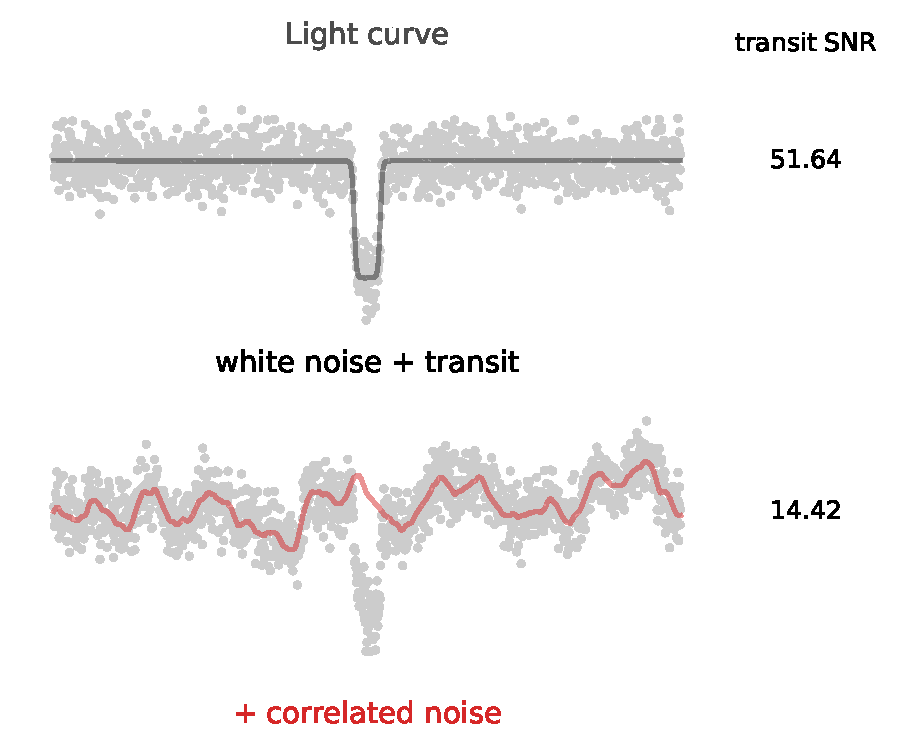
\includegraphics[width=8.5cm]{../figures/issue1.pdf}
        \caption{Illustration of the effect of correlated noise on a single transit singal-to-noise (SNR). A 1 hour transit of depth 1\% is simulated on top of white noise during a 24 hours observing window with an exposure time of 1 minute (top). Then, in the bottom plot, correlated noise is added to the transit signal and simulated using a Gaussian Process (GP) with a Matèrn-32 kernel of length-scale 1 hour and amplitude 0.2\%. The SNR on the right of each light curve is computed using \autoref{eq:snr}.}
        \label{fig:issue1}
    \end{centering}
\end{figure}

As illustrated in \autoref{fig:issue1}, the presence of correlated noise strongly decreases transit signals SNR, fundamentally limiting their detection. This issue rapidly motivated the development of systematics detrending algorithms such as the Trend Filtering Algorithm (\textsc{TFA}, \citealt{tfa}, in its primary use case), \textsc{SysRem} (\citealt{sysrem}), or Pixel Level Decorrelation (\textsc{PLD}, \citealt{pld}; see also \textsc{Everest} from \citealt{everest1, everest2}). Most of these methods rely on the shared nature of instrumental signals among light-curves (or neighboring pixels) such that the correction applied should not degrade the transit signal (in practice it does). We note that, except for \textsc{TFA}, these algorithms are mostly applied to space-based continuous observations, that provide continuous stellar baselines and mostly reproducible systematic signals. This is not the case for the vast majority of ground-based observations, in addition subject to periodic daytime interruptions and varying atmospheric extinction.

\subsection{The effect of detrending on transits detectability}

Instrumental signals have the benefit to be shared among light curves of stars observed with the same instrument, strongly correlated with measurements from the experimental setup (like detector's temperature, pointing error, sky background or airmass), hence we will make the strong assumption that their detrending based on an incomplete model of the light curve, one that ignore transit signals (because unknowns), do not affect the latter. In opposition, stellar variability is generally unknown and harder to correlate with simultaneous measurements. This gave rise to two types of treatments in order to reconstruct and detrend stellar variability, and perform transit search on \textit{flattened} light curves. One is physically-motivated and make use of Gaussian Processes (e.g. \cite{k2sc}). The other is empirical and make use of filtering algorithms (a wide variety being described in \cite{wotan}). In this section, we will study in details the effect of both approaches on transit detectability, by studying the degradation of a unique transit SNR for a wide variety of stellar variability characteristics.
\bigskip\\
Throughout this paper, we simulate stellar variability (and later model it) thanks to Gaussian Processes (GP), employing the physically-motivated stochastically-driven damped simple harmonic oscillator kernel (SHO) presented in \citealt{celerite1} (see Annexe ...). We generate stellar variability thanks to the \texttt{tinygp}\footnote{\href{https://github.com/dfm/tinygp}{https://github.com/dfm/tinygp}} Python package, providing an implententation of the scalable GP method from \citealt{celerite2} powered by \texttt{JAX}\footnote{\href{https://github.com/google/jax}{https://github.com/google/jax}}.

\begin{figure}[H]
    \begin{centering}
        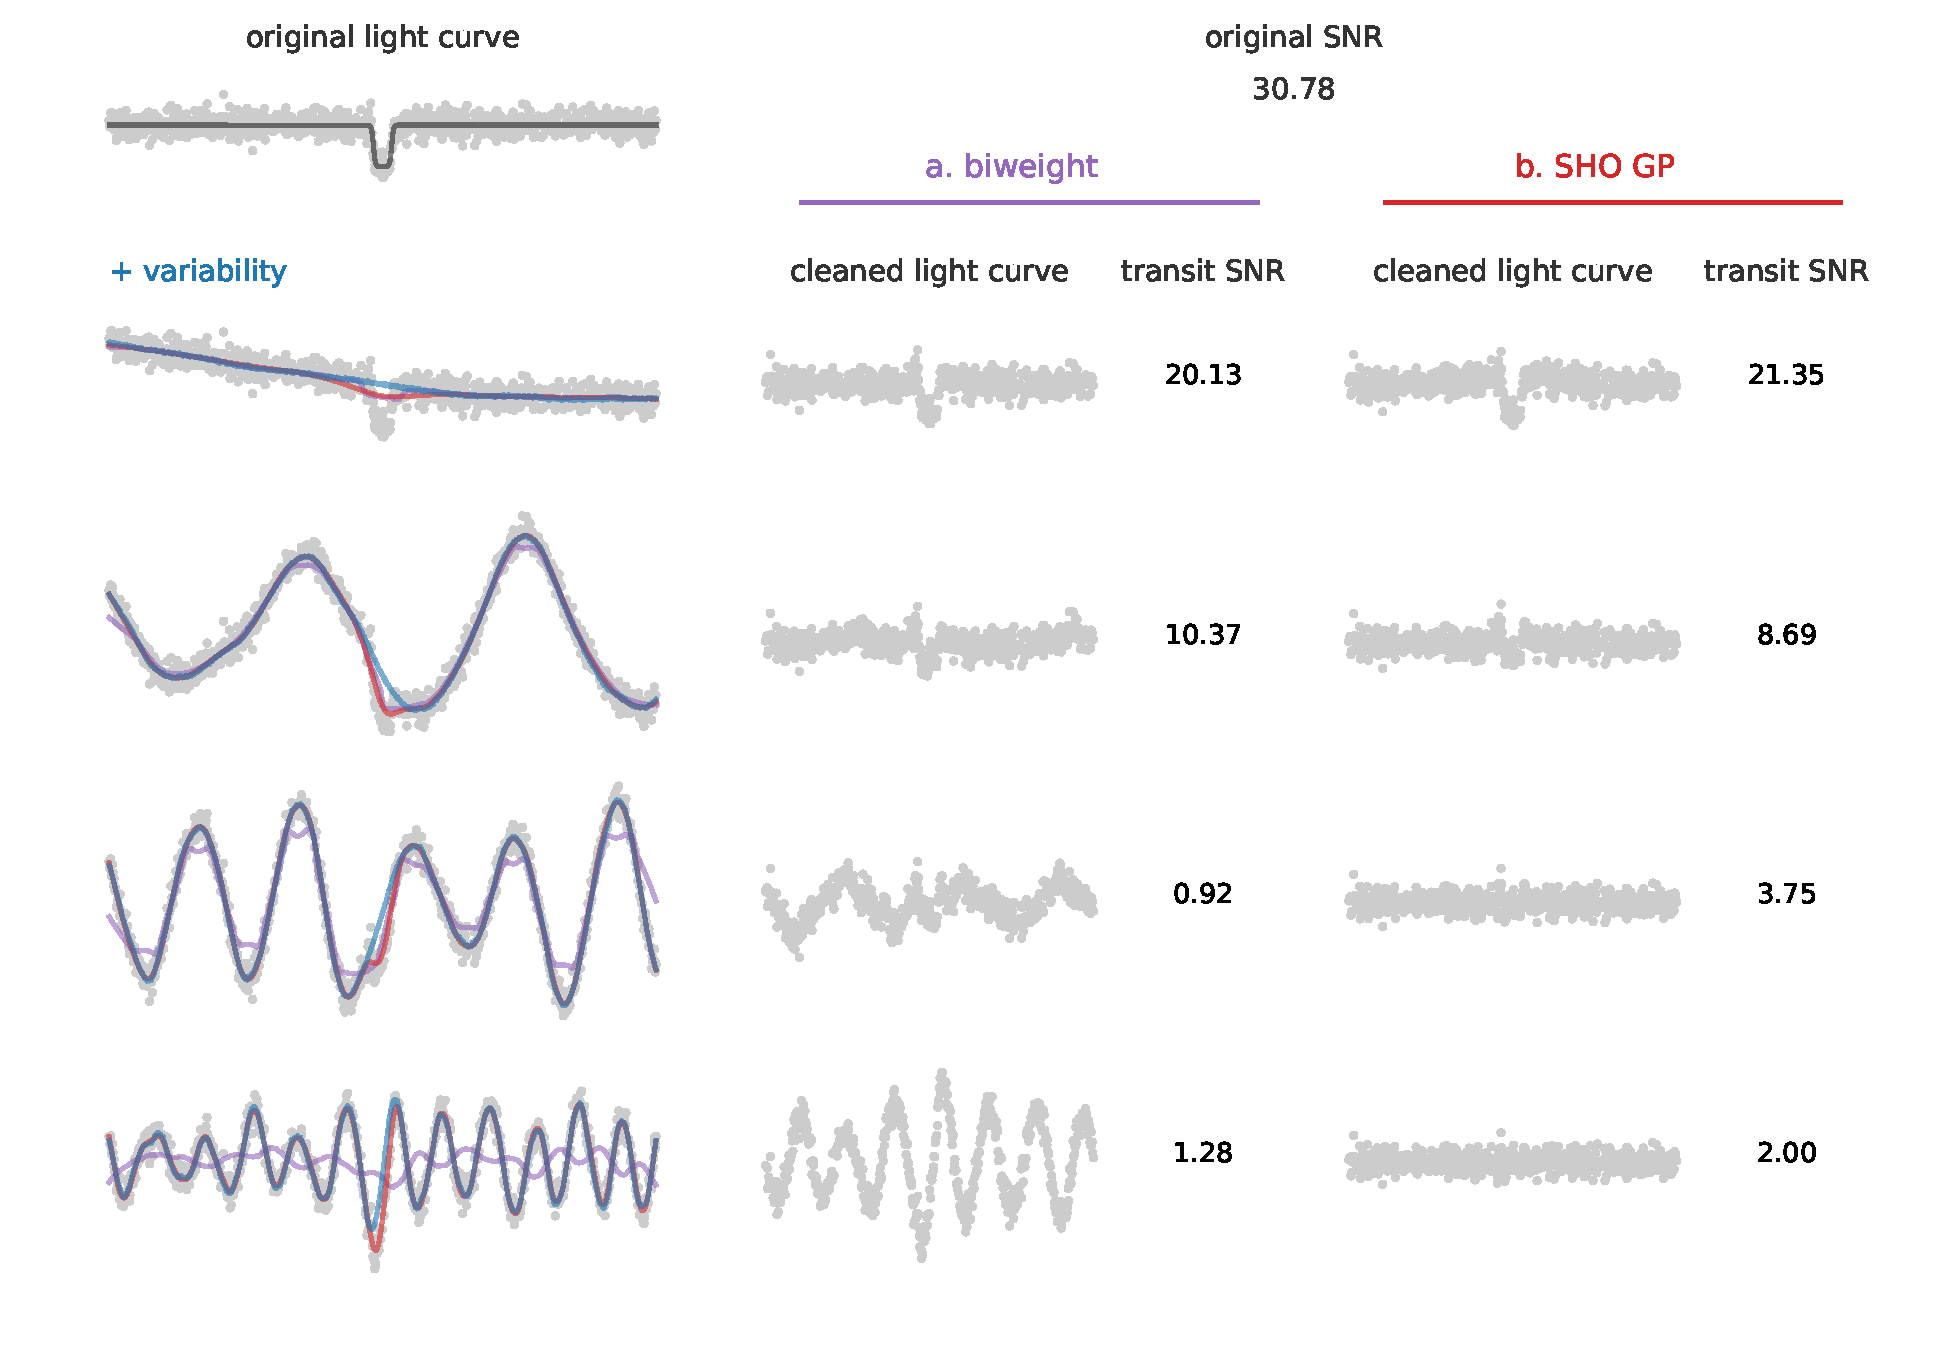
\includegraphics[width=\linewidth]{../figures/issue2.pdf}
        \caption{This is a pretty visualization of the Mandelbrot set.}
        \label{fig:issue2}
    \end{centering}
\end{figure}

In \autoref{fig:issue2}, we simulate a light curve featuring a single transit (again using the model from \citealt{protopapas}), in addition with stellar variability of different timescales and amplitudes. In case \textit{a} (purple in \autoref{fig:issue2}), we model and detrend these signals using the widely-adopted Tukey's biweight filtering method presented in \citealt{tukey} and its implementatation from \texttt{wõtan}\footnote{\href{https://github.com/hippke/wotan}{https://github.com/hippke/wotan}} \citep{wotan}. In case \textit{b} (red in \autoref{fig:issue2}) we employ the same GP model used to simulate stellar variability to reconstruct and remove it from light curves ignoring the presence of potential transits (the case of unknown transits search). Once transits cleaned from stellar variability, we asses their remaining SNR using \autoref{eq:snr}.
\bigskip\\
\autoref{fig:issue2} clearly shows the effect of both detrending techniques on transits SNR, and suggests that this degradation is strongly dependant on the stellar variability characteristics encountered. In order to explore the parameter space for which detrending is the most problematic, we simulate light curves including a single transit and a much wider range of correlated noise characteristics defined with two parameters: $\tau_v$ the relative timescale of the variability with respect to the transit duration; and $\delta_v$, the relative amplitude of the variability against transit depth, such that:

\begin{equation}
    \tau_v \propto \frac{\mathrm{variability\; timescale}}{\mathrm{transit\;duration}} \quad \text{and} \quad 
    \delta_v \propto \frac{\mathrm{variability\; amplitude}}{\mathrm{transit\;depth}} 
\end{equation}

To follow this parametrization, we simulate the photometric variability using a GP with an SHO kernel with hyperparameters \footnote{}:

\begin{equation}\label{eq:params}
    \omega = \frac{\pi}{\tau_v\tau} \quad 
    \sigma = \delta_v \frac{\delta^2}{4} \quad  \text{and}  \quad  
    Q = 10
\end{equation}

with $\delta$ and $\tau$ the depth and duration of the simulated transit, similar in all light curves. We fix a relatively high value for the quality factor $Q$ in order to restrict our simulations to strongly periodic variability signals. For $\tau_v=1$ and $\delta_v=1$, the expressions of $\omega$ and $\sigma$ given in \autoref{eq:params} correspond to a periodic signal with a period half that of the transit duration, and a peak to peak amplitude two times that of the transit depth, i.e. strongly resembling the simulated transit signal. As in \autoref{fig:issue2}, we reconstruct the variability using a biweight filter with a window length of $3\tau$ (three times the transit duration, an optimal value according to \citealt{wotan}). We then subtract the variability from each light-curve, estimate the resulting transit depth (using the in-transit minimum flux) and compute its SNR. \autoref{fig:snr_detrend} shows the remaining SNR values of transits computed this way, after each variability signals with random $(\tau_v, \delta_v)$ have been detrended.
\bigskip\\
\autoref{fig:snr_detrend} shows that it exists an entire region of the $(\tau_v, \delta_v)$ parameter space for which detrending degrades transit SNR to the point of no detection ($SNR < 6$). While this region might only represent a fraction of existing exoplanetary systems, we argue that these systems are of great value for the field of exoplanetary science. First, as variability is often linked to starspots co-rotation with their star, systems whose  with the stellar photo in is likely to be observed on stars whose equatorial plane lines up with our line of sight, following recent studies on the dynamical evolution of planetary systems \cite{}, hence being most likely to be transited. As a direct consequence, these same starspots are more likely to be occulted by planetary companions, events whose measurement benefits both the study of stellar atmospheres and their concerning impact on planetary atmospheric retrievals \cite{}. Finally, the growing interest of the community for ultra-cool dwarf stars comes with observations done in the infrared, featuring enhanced red noise and variability, leading to lower transit SNR \cite{}. Hence, commonly-used detrending technique (such as the biweight filter studied in this section) make transit-search blind to those pristine systems, motivating the need for a more informed transit search algorithm properly accounting for correlated noise. In the next section we present such an algorithm: \texttt{nuance}.

\begin{figure}[H]
    \begin{centering}
        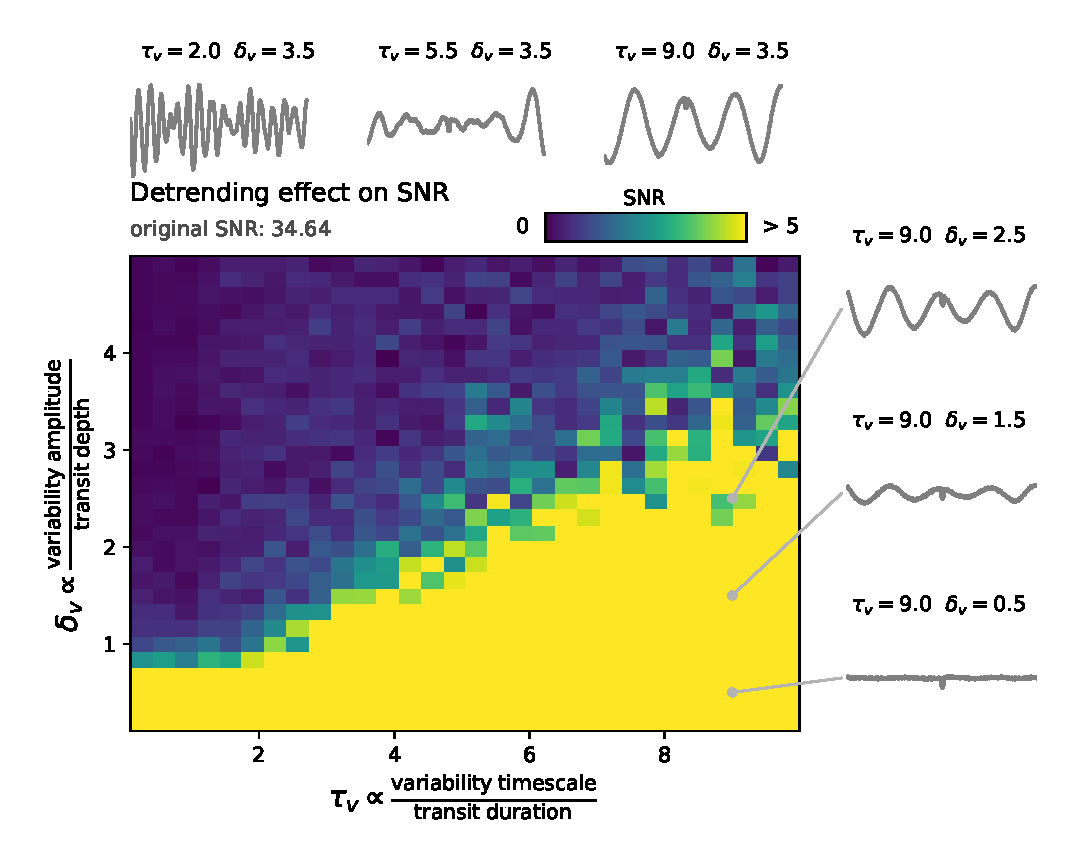
\includegraphics[height=10cm]{../../workflows/cleaning_snr/figures/simu1/result.pdf}
        \caption{This is a pretty visualization of the Mandelbrot set.}
        \label{fig:snr_detrend}
    \end{centering}
\end{figure}

\section{\texttt{nuance}}

\section{Injection-recovery on simulated data}

\begin{figure}[H]
    \begin{centering}
        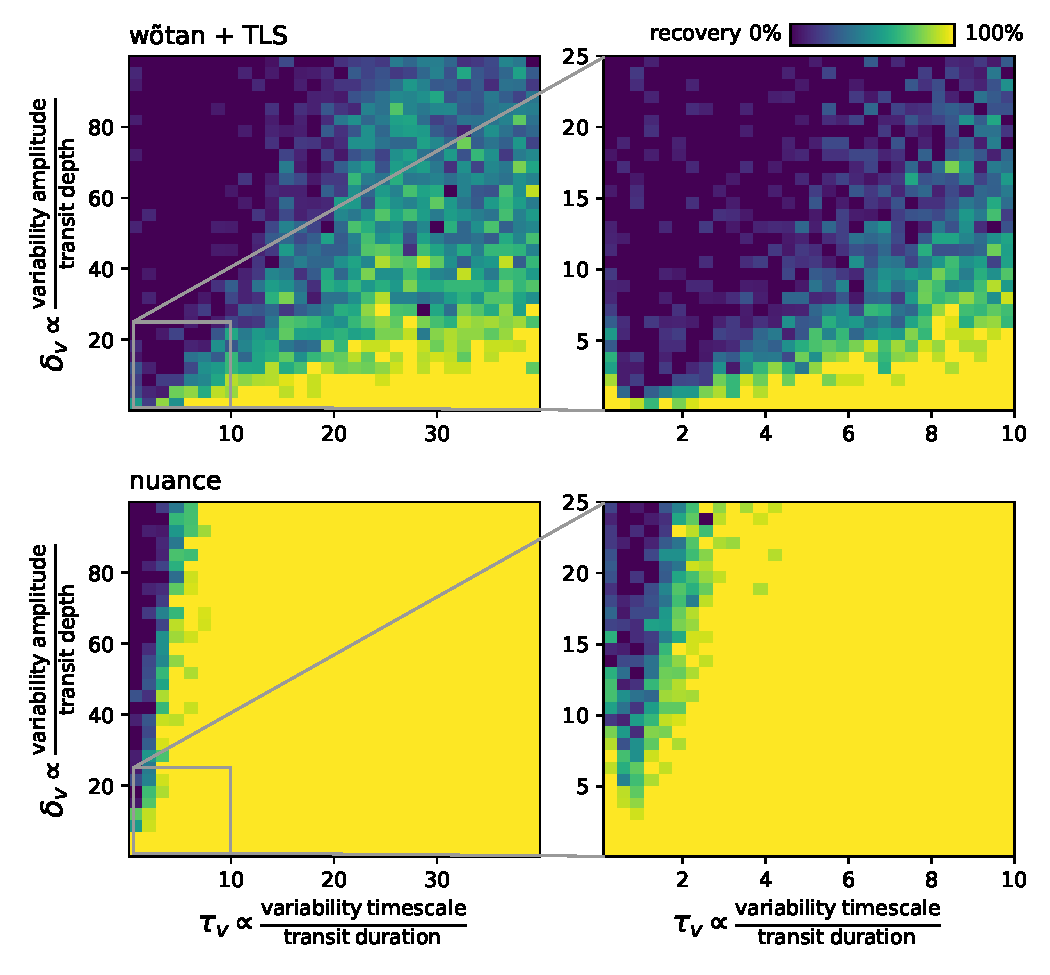
\includegraphics[height=12cm]{../../workflows/synthetic_injection_recovery/figures/final_result.pdf}
        \caption{This is a pretty visualization of the Mandelbrot set.}
        \label{fig:simu}
    \end{centering}
\end{figure}

\bibliography{bib}

\end{document}
